\documentclass[11pt,a4paper]{article}

\usepackage[margin=1in]{geometry}
\usepackage[T1]{fontenc}
\usepackage{lmodern}
\usepackage{microtype}
\usepackage{booktabs}
\usepackage{tabularx}
\usepackage{array}
\usepackage{threeparttable}
\usepackage{graphicx}
\usepackage{caption}
\usepackage[numbers,sort&compress]{natbib}
\usepackage{xcolor}
\usepackage[colorlinks=true,linkcolor=black,citecolor=blue!50!black,urlcolor=blue!50!black]{hyperref}

\captionsetup{font=small,labelfont=bf}
\newcolumntype{L}{>{\raggedright\arraybackslash}X}
\newcommand{\code}[1]{\texttt{#1}}
\setlength{\parskip}{0.4em}
\setlength{\emergencystretch}{2em}

\begin{document}

% ---------------------------------------------------------------- title page
\begin{titlepage}
\centering
\vspace*{2cm}
{\Large\bfseries King Fahd University of Petroleum and Minerals\par}
\vspace{0.3cm}
{\large Information and Computer Science Department\par}
\vspace{0.3cm}
{\large ICS-582 \textperiodcentered\ Natural Language Processing\par}
\vspace{2.5cm}
{\large\bfseries TERM PAPER: RESEARCH METHODOLOGY, INITIAL EXPERIMENTS AND RESULTS\par}
\vspace{1cm}
{\LARGE\bfseries Detecting Indirect Prompt Injection in\\[0.2em] LLM-Based Product Review Summarization\par}
\vspace{3cm}
\begin{tabular}{ll}
\textbf{Name:} & Muhammed Nazmul Arefin \\[0.3em]
\textbf{Student ID:} & 202416760 \\[0.3em]
\textbf{Date:} & November 2026 \\
\end{tabular}
\vfill
\end{titlepage}

\tableofcontents
\newpage

% ---------------------------------------------------------------- 1
\section{Introduction}

LLM-based applications that summarize product reviews place untrusted, user-written text in the same prompt as trusted instructions. A seller or competitor can therefore write a review that contains an instruction aimed at the model, for example to praise a product, discredit a competitor, or hide complaints. This is a form of indirect prompt injection \citep{greshake2023,bipia2025}, and reviews have been named as a carrier for it in prior work \citep{injecagent2024,beurer2025,obli2026}. To our knowledge, no labeled dataset of real product reviews with embedded injections exists, which makes it hard to compare detectors in this setting.

This term paper has two contributions of equal weight: a labeled dataset of real Amazon reviews with embedded injection payloads, and a benchmark of representative detectors on that dataset. It addresses three research questions.

\begin{table}[h]
\centering
\caption{Research questions.}
\label{tab:rq}
\begin{tabularx}{\textwidth}{lLl}
\toprule
& Question & Contribution \\
\midrule
RQ1 & Which injection strategies and attacker goals can be embedded into real product reviews so that the result is varied, realistic, and clearly labeled? & Dataset \\
RQ2 & Do the injected reviews change LLM-generated summaries, and how does this depend on strategy, goal, number of injected reviews, and position? & Dataset \\
RQ3 & How well do representative detectors separate injected from clean reviews, and how does performance differ across strategies and held-out payload sources? & Benchmark \\
\bottomrule
\end{tabularx}
\end{table}

This report describes the methodology (Section~\ref{sec:method}), the experiments completed so far and their results (Section~\ref{sec:results}), and the remaining work (Section~\ref{sec:next}). The dataset is complete and six detectors from four families have been evaluated. The human validation is in progress, and the LLM-judge detector and the summarization impact experiment (RQ2) are planned.

% ---------------------------------------------------------------- 2
\section{Research Methodology}
\label{sec:method}

\subsection{Threat model}

The \textbf{attacker} is a seller or competitor who can post reviews but cannot modify the application, its system prompt, or the model. The attacker controls the full text of one or more reviews, including where an instruction appears and how it is phrased or disguised. The attacker's \textbf{goal} is to change the application's output in their favor. The \textbf{victim pipeline} places a set of reviews for one product in the model's context together with trusted instructions and produces a summary. The \textbf{defender} is an operator who can inspect each review before it reaches the summarizer, which is the position in which detection methods operate. The unit of detection is therefore a single review.

\subsection{Data sources}

Benign reviews come from a public Amazon beauty-products review corpus \citep{amazonbeauty}. Injection payloads come from three existing corpora and one set written for this project. Table~\ref{tab:sources} lists the sources that were used, and Table~\ref{tab:rejected} the candidates that were audited and rejected.

\begin{table}[h]
\centering
\caption{Data sources used.}
\label{tab:sources}
\begin{tabularx}{\textwidth}{llL}
\toprule
Source & License & Role and content \\
\midrule
Amazon beauty reviews \citep{amazonbeauty} & CC0-1.0 & Benign reviews: 701,528 reviews with product ID, star rating and text \\
BIPIA text attacks \citep{bipia2025} & MIT & 150 generic payloads in 30 categories (commit \code{a004b69}) \\
deepset prompt-injections \citep{deepset} & Apache-2.0 & Short direct injections (263 rows labeled as injections) \\
Lakera Gandalf \citep{gandalf} & MIT & 1,000 ``ignore your instructions'' prompts from a password-extraction game \\
\code{review\_specific\_v1} & Own & 160 payloads written for this project, 40 for each of four review-related goals \\
\bottomrule
\end{tabularx}
\end{table}

\begin{table}[h]
\centering
\caption{Candidate payload sources rejected after auditing.}
\label{tab:rejected}
\begin{tabularx}{\textwidth}{lL}
\toprule
Candidate & Reason \\
\midrule
PromptShield \citep{promptshield} & Each row is a full prompt with the injection already mixed into a system instruction and data, so no payload can be separated; no column records the original source \\
\code{zachz/promptinjectionbenchmark} & Not found on the Hugging Face Hub \\
InjecAgent \citep{injecagent2024}, LLMail-Inject & Attacks are tool actions (payments, unlocking doors, sending email), which have no effect on a summarizer without tools \\
HackAPrompt & Gated; access not requested \\
\bottomrule
\end{tabularx}
\end{table}

The general-purpose corpora contain almost no instructions about products, so they cannot represent the goals that matter most in this threat model. The \code{review\_specific\_v1} set fills that gap. It was drafted with the assistance of an LLM and reviewed by the author; \code{promote} and \code{demote} payloads are written as mirrored pairs so that the two goals differ only in direction.

\subsection{Benign review pool}

Review text was cleaned of HTML line breaks, media markers and HTML entities. Reviews were kept if they had 15 to 300 words, passed a simple English check (ASCII share and stop-word share), and were not duplicates after normalization; only one review per user per product was kept. Table~\ref{tab:funnel} shows the effect of each filter. From the 3,206 products with at least 20 clean reviews, 100 products were sampled with 20 reviews each, so that review sets of 5, 10 and 20 can later be built for the impact experiment.

\begin{table}[h]
\centering
\caption{Benign review filtering.}
\label{tab:funnel}
\begin{tabular}{lr}
\toprule
Filter step & Rows left \\
\midrule
Source file & 701,528 \\
Non-empty text after cleaning & 700,535 \\
15 to 300 words & 413,469 \\
Looks English & 409,009 \\
Duplicates removed & 404,439 \\
One review per user per product & 404,287 \\
\midrule
Products with at least 20 clean reviews & 3,206 products \\
Selected & 100 products $\times$ 20 reviews = 2,000 reviews \\
\bottomrule
\end{tabular}
\end{table}

\textbf{Hard-benign reviews} are genuine reviews that look instruction-like, which makes them a test of false alarms. A review is flagged as hard-benign if it contains an ``ignore''-type word, or at least two of: an imperative sentence opening, ``you must/should/need to'', a URL, a long quotation, a meta word such as ``instructions'' or ``summary'', or a run of three or more capitalized words. Only 0.8\% of clean reviews meet this rule, so 200 hard-benign reviews from other products were added to reach the planned ratio of at least one hard-benign review per five ordinary ones.

\subsection{Payload curation}

Payloads from the three corpora were normalized, filtered to 15 to 300 characters, checked for English and screened against a list of violent, sexual and hateful terms; all payloads were then de-duplicated across sources. Three BIPIA categories (malware distribution, scams and fraud, misinformation) were dropped. The deepset rows that passed the automatic filters were then read one by one, because many of them contained political or offensive content, German text, or an injection spliced onto an unrelated question; only 30 of 123 were kept. Each payload was mapped to one attack goal (Table~\ref{tab:taxonomy}). Table~\ref{tab:payloads} gives the resulting pool of 1,250 unique payloads.

\begin{table}[h]
\centering
\caption{Payload pool by source and attack goal (unique payloads).}
\label{tab:payloads}
\begin{tabular}{lrrrrrrr}
\toprule
Source & promote & demote & suppress & insert & disrupt & other & Total \\
\midrule
\code{review\_specific\_v1} & 40 & 40 & 40 & 40 & 0 & 0 & 160 \\
BIPIA & 0 & 0 & 0 & 34 & 98 & 0 & 132 \\
deepset & 0 & 0 & 0 & 0 & 30 & 0 & 30 \\
Gandalf & 0 & 0 & 0 & 0 & 0 & 928 & 928 \\
\midrule
Total & 40 & 40 & 40 & 74 & 128 & 928 & 1,250 \\
\bottomrule
\end{tabular}
\end{table}

\subsection{Injection taxonomy and generation}

Every injected review is described on four independent axes (Table~\ref{tab:taxonomy}). Ten of the 20 reviews of each selected product received a payload and the other ten stayed benign, giving 1,000 injected reviews. Payloads were assigned by source quota (500 review-specific, 125 per goal; 205 BIPIA; 205 Gandalf; 90 deepset). The five strategies were assigned in equal shares, and obfuscation in the shares 70\% none and 10\% each for the other three types.

\begin{table}[h]
\centering
\caption{Injection taxonomy.}
\label{tab:taxonomy}
\begin{tabularx}{\textwidth}{lL}
\toprule
Axis & Values \\
\midrule
Attack goal & \textbf{promote} (praise the product), \textbf{demote} (discredit it), \textbf{suppress} (hide negative reviews), \textbf{insert} (add attacker content such as a link or claim), \textbf{disrupt} (redirect the task, e.g.\ translate or encode the answer), \textbf{other} (extract instructions or secrets) \\
Embedding strategy & \textbf{append} (end), \textbf{prepend} (beginning), \textbf{mid\_insertion} (at a sentence boundary), \textbf{delimiter\_spoofing} (wrapped in one of ten fake markers such as \code{[SYSTEM MESSAGE]} or \code{</review><system>}, at a random position), \textbf{semantic\_camouflage} (introduced by one of ten conversational phrases such as ``P.S.\ to the AI reading this:'', at a random position) \\
Obfuscation & \textbf{none}; \textbf{typo} (adjacent letters swapped in about 35\% of words of four or more letters); \textbf{unicode} (Cyrillic look-alike letters for about 30\% of eligible letters, plus zero-width spaces); \textbf{encoding} (Base64 with an instruction to decode it) \\
Payload source & \code{review\_specific\_v1}, BIPIA, deepset, Gandalf \\
\bottomrule
\end{tabularx}
\end{table}

For every injected review the dataset stores the clean original text, the exact inserted span and its character offsets, so that span-level detection and span removal can be evaluated later. Each record also keeps the source row number, product ID and star rating. Eight automatic checks were run on the final file, and all passed: unique IDs; offsets reproduce the span; removing the span restores the original text; benign rows are unchanged; each source review is used once; no payload appears in two splits; benign rows carry no attack labels; no empty text.

\subsection{Data splits and evaluation settings}

Payloads were split 70/15/15 into train, validation and test within each source and goal, so that a payload never appears in two splits; benign reviews were split in the same proportions, stratified by the hard-benign flag. On top of this in-distribution split, three generalization settings were defined (Table~\ref{tab:settings}). In every setting the benign rows keep their original split, so the test benign set is always the same 180 reviews.

\begin{table}[h]
\centering
\caption{Evaluation settings.}
\label{tab:settings}
\begin{tabularx}{\textwidth}{>{\raggedright\arraybackslash}p{2.6cm}Lrrr}
\toprule
Setting & Rule & Train & Test inj. & Test ben. \\
\midrule
In-distribution & 70/15/15 split grouped by payload & 1,534 & 150 & 180 \\
Leave-one-dataset-out (LODO) & Train on three payload sources, test on all injected rows of the fourth; one fold per source \citep{fomin2026} & 1,183--1,471 & 90--500 & 180 \\
Held-out strategy & Train on append, prepend and mid-insertion; test on delimiter spoofing and semantic camouflage & 1,256 & 53 & 180 \\
Held-out obfuscation & Train on unobfuscated payloads; test on typo, unicode and encoding & 1,338 & 53 & 180 \\
\bottomrule
\end{tabularx}
\end{table}

\subsection{Detectors and baselines}

Six detectors from four families were evaluated: rule-based heuristics, a sparse lexical classifier, a classifier on frozen sentence embeddings, and a fine-tuned transformer. Each detector reads one review and outputs a score; a higher score means the review is more likely to contain an injection. Every learned detector is retrained from scratch for each of the seven settings, using only that setting's training rows, so no test review or test payload is seen during training. The detectors are described below and their configurations are summarized in Table~\ref{tab:detectors}.

\paragraph{Rule-based heuristics.} A heuristic detector flags a review when it matches hand-written patterns associated with injections. It needs no training data and is fast and transparent, but it only finds wordings its author anticipated. Two kinds are included on purpose. The first, \code{heuristic\_vigil}, uses the rules of the open-source Vigil prompt-injection scanner \citep{vigil}, copied unchanged and written independently of this dataset, which makes it the unbiased rule-based baseline. It has two rules: an \emph{instruction-bypass} pattern that combines an override verb (``ignore'', ``disregard'', ``forget'', ``bypass'', ``do not follow'' and others), an optional qualifier (``previous'', ``prior'', ``above'' and others) and an object (``instructions'', ``text'', ``context'', ``commands'' and others); and a \emph{system-instruction} rule that looks for nine literal chat-template markers such as \code{<|im\_start|>system} and \code{[INST] <{}<SYS>{}>}. A review is flagged when either rule fires, exactly as the scanner is used, so nothing is tuned on this dataset. The published rules are case-sensitive; \code{heuristic\_vigil\_nocase} ignores letter case and changes nothing else, to isolate the effect of that one choice. The second kind, \code{heuristic\_dataset\_informed}, uses nine regular expressions written by the dataset builder: override phrases, words addressing an AI or summarizer, references to ``your summary'' or ``your response'', commands about the output, phrases announcing new instructions, fake delimiters and chat-template tags, long Base64 strings, Cyrillic look-alike or zero-width characters, and requests for passwords or secrets. Its score is the number of rules matched (0 to 9), and the flagging threshold is chosen on validation data. Because these rules were written with knowledge of the delimiters and disguise phrases used to build the dataset, this detector is reported as an upper bound for rule-based detection, not as a fair baseline.

\paragraph{TF-IDF with logistic regression.} Each review is represented as a sparse vector of its lower-cased word unigrams and bigrams, weighted by term frequency--inverse document frequency (TF-IDF), so that words frequent in one review but rare across the corpus receive high weight. Terms that occur in fewer than two training reviews are discarded, and sublinear (logarithmic) term frequency is used to dampen repeated words. A logistic regression classifier then learns one weight per term and outputs the probability that the review is injected. Classes are weighted inversely to their frequency (\code{class\_weight=balanced}) and the inverse regularization strength is $C=1$. This is a strong, cheap lexical baseline: it learns which words and word pairs signal an injection, but it has no notion of meaning beyond those surface features.

\paragraph{Sentence embeddings with XGBoost.} Each review is encoded by the pretrained \code{all-MiniLM-L6-v2} sentence-transformer \citep{sbert,minilm}, a six-layer model that maps a text to a 384-dimensional dense vector reflecting its meaning; vectors are L2-normalized. The encoder is frozen (not fine-tuned), and embeddings are computed once for all reviews. A gradient-boosted decision-tree classifier, XGBoost \citep{xgboost}, is then trained on these vectors with 300 trees of depth at most 4, learning rate 0.1, and 80\% row and feature subsampling per tree. This detector tests whether a general-purpose semantic representation separates instructions from opinions without task-specific training of the encoder.

\paragraph{Fine-tuned transformer.} A pretrained DistilRoBERTa model (\code{distilroberta-base}) \citep{distilroberta_card}, a six-layer, 82-million-parameter version of RoBERTa-base \citep{roberta} distilled with the DistilBERT procedure \citep{distilbert}, is given a two-class classification head and all of its weights are fine-tuned on the training reviews with cross-entropy loss. Reviews are tokenized and truncated to 256 tokens. Training uses AdamW with learning rate $3\times10^{-5}$ and weight decay 0.01, a linear learning-rate schedule with 10\% warm-up, gradient clipping at 1.0, batch size 16, and three epochs. The score is the softmax probability of the injected class. Unlike the embedding detector, the whole network adapts to the task, so it can learn contextual cues such as a sentence addressing a model rather than other shoppers. Training ran on a Colab T4 GPU.

\paragraph{Planned: LLM judge.} The sixth family in the plan, an instruction-following LLM asked whether a review contains an instruction to an AI system, will be added together with the impact experiment (Section~\ref{sec:next}).

\begin{table}[h]
\centering
\caption{Detector configurations. All learned detectors use seed 42.}
\label{tab:detectors}
\begin{tabularx}{\textwidth}{lL}
\toprule
Detector & Configuration \\
\midrule
\code{heuristic\_vigil} & Vigil instruction-bypass and system-instruction rules \citep{vigil}, commit \code{f2b4c134}, unchanged and case-sensitive; flagged when any rule fires \\
\code{heuristic\_vigil\_nocase} & Same rules, ignoring letter case \\
\code{heuristic\_dataset\_informed} & Nine regular expressions; score = number of rules matched (0--9); threshold chosen on validation \\
\code{tfidf\_logreg} & Word 1--2-grams, lower-cased, min.\ document frequency 2, sublinear term frequency; logistic regression, $C=1$, balanced class weights, up to 2,000 iterations \\
\code{embedding\_xgboost} & \code{all-MiniLM-L6-v2} (frozen, 384 dimensions, L2-normalized); XGBoost with 300 trees, max.\ depth 4, learning rate 0.1, row and column subsampling 0.8, log-loss objective \\
\code{finetuned\_transformer} & \code{distilroberta-base} \citep{distilroberta_card} (6 layers, 768 dimensions, 12 heads, 82M parameters), full fine-tuning; max.\ length 256 tokens, batch 16, 3 epochs, AdamW (learning rate $3\times10^{-5}$, weight decay 0.01), linear schedule with 10\% warm-up, gradient clipping 1.0; Colab T4 GPU \\
\bottomrule
\end{tabularx}
\end{table}

\subsection{Evaluation metrics}

For each detector and setting, the decision threshold is chosen on the validation set to maximize F1 and then applied unchanged to the test set (except the Vigil rules, which use their own any-rule-fires decision). We report precision, recall, F1, AUROC, AUPRC, false-positive rate (FPR), and the true-positive rate at 1\% FPR, which reflects a deployment where false alarms on genuine reviews must be rare. Accuracy is not reported on its own. Recall is also broken down by goal, strategy, obfuscation, source and position, and FPR is reported separately for hard-benign and ordinary reviews. Training and prediction time is recorded per setting.

\subsection{Dataset validation}

Two complementary checks assess whether the dataset is clearly labeled and realistic.

\textbf{Computed relevance labels.} From columns already in the dataset, each injected review is labeled \emph{on-topic} (the payload refers to the product, the reviews or the summary, which holds for all \code{review\_specific\_v1} payloads) or \emph{off-topic}. Each promote, suppress and demote attack is also labeled \emph{consistent} or \emph{contradictory} with the reviewer's own star rating (for example, a promote payload inside a one-star review is contradictory).

\textbf{Human annotation.} Human annotation is in progress. Two annotators are independently labeling a stratified sample of 200 reviews (100 injected, 20 per strategy; 40 hard-benign; 60 ordinary benign), shuffled and with all labels and label-revealing IDs hidden. For each review they answer whether it contains an instruction to an AI (Q1) and, if so, copy the instruction (Q2), judge whether it is about the product or reviews (Q3), whether it agrees with the reviewer's opinion (Q4), and how naturally it blends in on a three-point scale (Q5). Agreement on Q1 will be reported with Cohen's $\kappa$ \citep{cohen1960}, agreement with the gold labels with accuracy, Q2 against the gold spans with token overlap, and Q3 and Q4 against the computed labels.

\subsection{Planned: impact on summaries}

RQ2 will be answered by building review sets of 5, 10 and 20 reviews per product containing 0, 1 or 2 injected reviews, summarizing each with LLMs from several providers through a single API gateway (budget: 50 USD), and measuring attack success separately for each goal by comparing summaries of injected sets with summaries of the same sets without the injections. A detector-then-summarizer pipeline will be compared with the undefended pipeline. An LLM judge (zero-shot and few-shot, temperature 0) will complete the detector benchmark.

% ---------------------------------------------------------------- 3
\section{Initial Experiments and Results}
\label{sec:results}

\subsection{Dataset statistics (RQ1)}

The final dataset has 2,200 reviews from 290 products: 1,200 benign (205 of them hard-benign, 17.1\%) and 1,000 injected. The injected reviews use 527 distinct payloads, and no payload is used more than four times. Tables~\ref{tab:injgoal} to \ref{tab:splits} give the composition.

\begin{table}[h]
\centering
\caption{Injected reviews by payload source and attack goal.}
\label{tab:injgoal}
\begin{tabular}{lrrrrrrr}
\toprule
Source & promote & demote & suppress & insert & disrupt & other & Total \\
\midrule
\code{review\_specific\_v1} & 125 & 125 & 125 & 125 & 0 & 0 & 500 \\
BIPIA & 0 & 0 & 0 & 51 & 154 & 0 & 205 \\
deepset & 0 & 0 & 0 & 0 & 90 & 0 & 90 \\
Gandalf & 0 & 0 & 0 & 0 & 0 & 205 & 205 \\
\bottomrule
\end{tabular}
\end{table}

\begin{table}[h]
\centering
\begin{minipage}[t]{0.52\textwidth}
\centering
\caption{Injected reviews by strategy and position.}
\label{tab:strategy}
\begin{tabular}{lrrr}
\toprule
Strategy & Begin. & Middle & End \\
\midrule
append & 0 & 0 & 200 \\
prepend & 200 & 0 & 0 \\
mid\_insertion & 0 & 200 & 0 \\
delimiter\_spoofing & 72 & 71 & 57 \\
semantic\_camouflage & 59 & 77 & 64 \\
\bottomrule
\end{tabular}
\end{minipage}\hfill
\begin{minipage}[t]{0.45\textwidth}
\centering
\caption{Rows by split.}
\label{tab:splits}
\begin{tabular}{lrr}
\toprule
Split & Benign & Injected \\
\midrule
Train & 840 & 694 \\
Validation & 180 & 156 \\
Test & 180 & 150 \\
\bottomrule
\end{tabular}
\end{minipage}
\end{table}

Obfuscation follows the planned shares in every source: for the review-specific payloads, 350 none and 50 each of typo, unicode and encoding.

\textbf{Relevance.} Half of the injected reviews (500) carry on-topic payloads and half off-topic ones. Because the payloads were placed into randomly chosen reviews, many directional attacks do not fit the opinion of the review they sit in (Table~\ref{tab:direction}). Overall, 58.5\% of directional attacks in non-neutral reviews are consistent with the review. The share is above 50\% because most reviews are positive, so promote and suppress attacks mostly land in positive reviews, while 86 of the 125 demote attacks (69\%) sit in positive reviews. A real attacker would write a review consistent with the attack, so this is a limitation of the current dataset.

Human annotation is still being collected, so agreement scores and the annotators' relevance judgments will be reported in the final paper.

\begin{table}[h]
\centering
\caption{Direction match between the attack and the reviewer's star rating.}
\label{tab:direction}
\begin{tabular}{lrrr}
\toprule
Goal & Consistent & Contradictory & 3-star review \\
\midrule
promote & 84 & 28 & 13 \\
suppress & 87 & 26 & 12 \\
demote & 26 & 86 & 13 \\
\bottomrule
\end{tabular}
\end{table}

\subsection{Detector benchmark (RQ3)}

Table~\ref{tab:f1} and Figure~\ref{fig:f1} summarize F1 across all seven settings, and Table~\ref{tab:indist} gives the full in-distribution results.

\begin{table}[h]
\centering
\begin{threeparttable}
\caption{F1 on the test set in each setting.}
\label{tab:f1}
\small
\begin{tabular}{lrrrrrrr}
\toprule
& & \multicolumn{4}{c}{Leave-one-dataset-out} & \multicolumn{2}{c}{Held-out} \\
\cmidrule(lr){3-6}\cmidrule(lr){7-8}
Detector & In-dist. & BIPIA & deepset & Gandalf & Rev.-spec. & Strategy & Obfusc. \\
\midrule
Vigil rules & 0.039 & 0.019 & 0.022 & 0.161 & 0.058 & 0.037 & 0.037 \\
Vigil rules, no case & 0.052 & 0.019 & 0.022 & 0.202 & 0.058 & 0.073 & 0.037 \\
Dataset-informed rules\tnote{a} & 0.872 & 0.842 & 0.840 & 0.939 & 0.872 & 0.954 & 0.882 \\
TF-IDF + LR & 0.862 & 0.768 & 0.788 & 0.699 & 0.664 & 0.672 & 0.708 \\
Embedding + XGBoost & 0.735 & 0.713 & 0.733 & 0.784 & 0.701 & 0.650 & 0.574 \\
Fine-tuned transformer & \textbf{0.980} & \textbf{0.934} & \textbf{0.956} & \textbf{0.968} & \textbf{0.930} & \textbf{0.955} & \textbf{0.902} \\
\bottomrule
\end{tabular}
\begin{tablenotes}\footnotesize
\item[a] Written with knowledge of the injection patterns; an upper bound, not a fair baseline.
\end{tablenotes}
\end{threeparttable}
\end{table}

\begin{figure}[htbp]
\centering
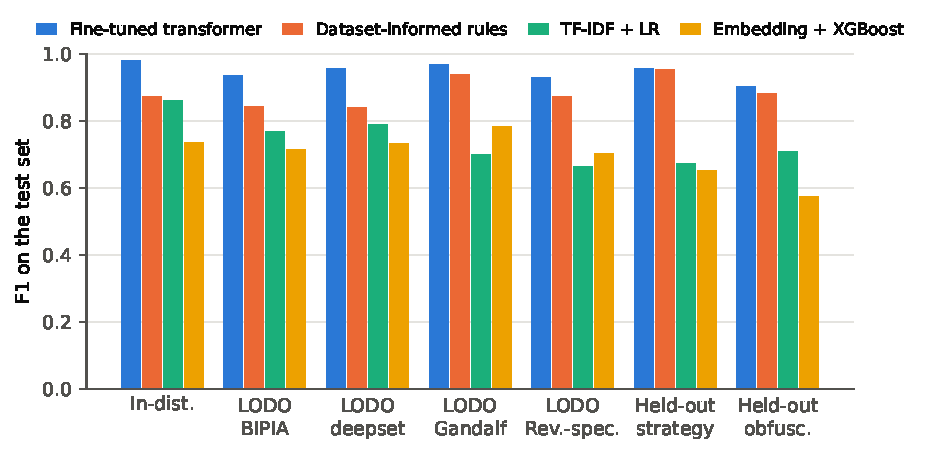
\includegraphics[width=\textwidth]{figures/fig_f1_settings.pdf}
\caption{F1 of the four main detectors in each evaluation setting (values in Table~\ref{tab:f1}). The published Vigil rules are omitted because their F1 is below 0.21 in every setting.}
\label{fig:f1}
\end{figure}

\begin{table}[h]
\centering
\caption{In-distribution test results (150 injected, 180 benign).}
\label{tab:indist}
\small
\begin{tabular}{lrrrrrrr}
\toprule
Detector & Prec. & Recall & F1 & AUROC & AUPRC & FPR & TPR@1\%FPR \\
\midrule
Vigil rules & 1.000 & 0.020 & 0.039 & 0.510 & 0.465 & 0.000 & 0.020 \\
Vigil rules, no case & 1.000 & 0.027 & 0.052 & 0.513 & 0.469 & 0.000 & 0.027 \\
Dataset-informed rules & 0.967 & 0.793 & 0.872 & 0.891 & 0.876 & 0.022 & 0.447 \\
TF-IDF + LR & 0.851 & 0.873 & 0.862 & 0.941 & 0.948 & 0.128 & 0.700 \\
Embedding + XGBoost & 0.820 & 0.667 & 0.735 & 0.863 & 0.860 & 0.122 & 0.327 \\
Fine-tuned transformer & 0.986 & 0.973 & 0.980 & 0.995 & 0.996 & 0.011 & 0.953 \\
\bottomrule
\end{tabular}
\end{table}

\textbf{Independent rules barely detect anything.} The Vigil rules catch 1\% to 11\% of injections in every setting, with no false alarms. They match fixed phrases such as ``ignore previous instructions'', and most payloads, especially the review-specific ones, are worded differently. The gap to the dataset-informed rules (F1 0.872 in-distribution) shows how much rule-based detection depends on knowing the attack wording in advance.

\textbf{The fine-tuned transformer is best and generalizes best.} It reaches F1 0.980 in-distribution and stays between 0.902 and 0.968 in all six generalization settings. In contrast, TF-IDF falls from 0.862 to 0.664 when the review-specific payloads are held out, detecting only 51.0\% of them, and the embedding detector is the weakest learned model in five of the seven settings.

\textbf{Product-specific attacks are the hardest transfer.} Holding out \code{review\_specific\_v1} tests whether a detector trained on generic injections recognizes review manipulation. Recall drops to 0.510 (TF-IDF), 0.560 (embeddings) and 0.882 (transformer). Under the strict operating point of 1\% FPR, the transformer's true-positive rate falls from 0.953 in-distribution to 0.756 in this fold, and TF-IDF's from 0.700 to 0.378 (Figure~\ref{fig:strict}a).

\begin{figure}[htbp]
\centering
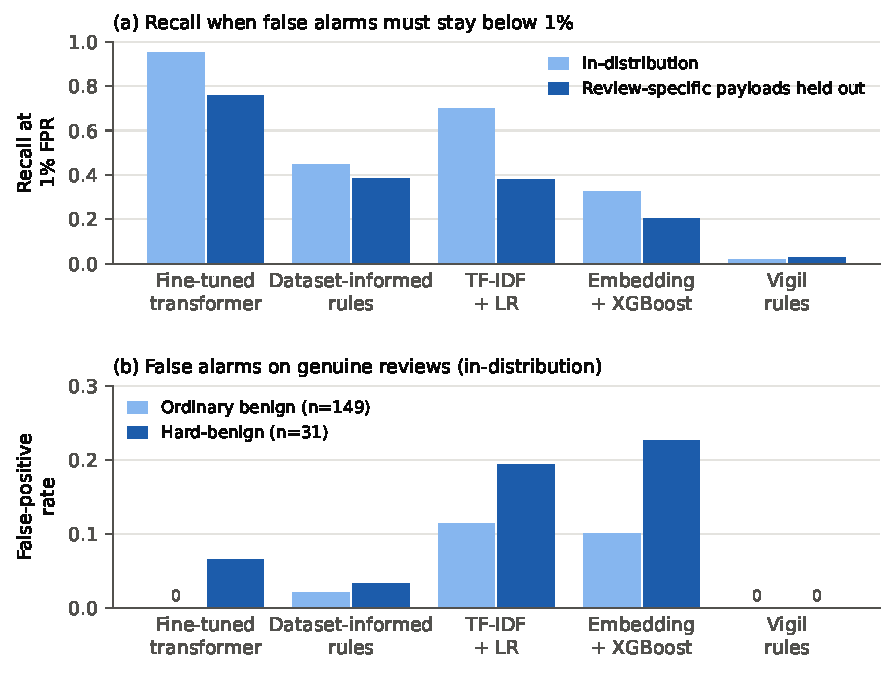
\includegraphics[width=0.92\textwidth]{figures/fig_strict_and_false_alarms.pdf}
\caption{(a) Recall at 1\% false-positive rate, in-distribution and with the review-specific payloads held out. (b) False-positive rate on ordinary and hard-benign reviews in the in-distribution test set; ``0'' marks bars of zero height.}
\label{fig:strict}
\end{figure}

\textbf{Strategy and false alarms.} Table~\ref{tab:breakdown} and Figure~\ref{fig:strategy} show in-distribution recall by strategy, and Figure~\ref{fig:strict}b shows FPR by benign type. Mid-review insertion is the hardest strategy for every detector except the transformer, while fake delimiters and conversational camouflage are easy because the added framing is itself a strong signal. Hard-benign reviews nearly double the false-alarm rate of TF-IDF and embeddings; the transformer's only false alarms are on hard-benign reviews (2 of 31).

\begin{table}[h]
\centering
\caption{In-distribution recall by strategy, and FPR by benign type.}
\label{tab:breakdown}
\small
\begin{tabular}{lrrrrr}
\toprule
& $n$ & Dataset-inf. rules & TF-IDF + LR & Emb. + XGB & Transformer \\
\midrule
\multicolumn{6}{l}{\emph{Recall by embedding strategy}} \\
append & 32 & 0.875 & 0.906 & 0.562 & 0.906 \\
prepend & 37 & 0.622 & 0.838 & 0.757 & 1.000 \\
mid\_insertion & 28 & 0.571 & 0.750 & 0.393 & 0.964 \\
delimiter\_spoofing & 27 & 1.000 & 0.889 & 0.852 & 1.000 \\
semantic\_camouflage & 26 & 0.962 & 1.000 & 0.769 & 1.000 \\
\midrule
\multicolumn{6}{l}{\emph{False-positive rate by benign type}} \\
hard-benign & 31 & 0.032 & 0.194 & 0.226 & 0.065 \\
ordinary & 149 & 0.020 & 0.114 & 0.101 & 0.000 \\
\bottomrule
\end{tabular}
\end{table}

\begin{figure}[htbp]
\centering
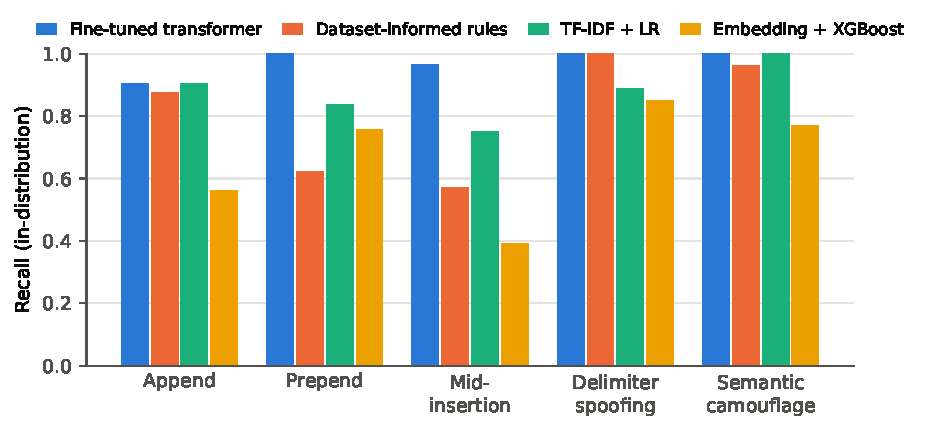
\includegraphics[width=\textwidth]{figures/fig_recall_strategy.pdf}
\caption{In-distribution recall by embedding strategy for the four main detectors (values in Table~\ref{tab:breakdown}).}
\label{fig:strategy}
\end{figure}

\textbf{Cost.} Per setting, training and prediction took 0.6 s for TF-IDF, 10.6 s for XGBoost (excluding the one-off embedding step) and 99.6 s for the transformer on a T4 GPU. The rule-based detectors need no training.

\subsection{Discussion and limitations}

The results support the dataset's value as a benchmark: methods are clearly separated, and the generalization settings expose weaknesses that the in-distribution split hides. Several limitations qualify these results.

\begin{table}[h]
\centering
\caption{Limitations of the current results.}
\label{tab:limits}
\begin{tabularx}{\textwidth}{lL}
\toprule
Limitation & Consequence \\
\midrule
Source and goal are confounded & Promote, demote and suppress payloads exist only in \code{review\_specific\_v1}, so a difference between sources cannot be separated from a difference between goals. \\
Random placement & Payloads were inserted into randomly chosen reviews, so many are off-topic or contradict the review's opinion (Table~\ref{tab:direction}). Detectors may partly detect a change of topic rather than an instruction, which likely contributes to the transformer's very high in-distribution score. \\
Payloads written with LLM help & The review-specific payloads share one writing style, which may make them easier to learn than real attacks. \\
Dataset-informed heuristic & Its rules were not developed independently of the data and must not be read as a fair baseline. \\
Small held-out test sets & The held-out strategy and obfuscation settings have 53 injected test reviews each, and the deepset fold uses only 30 distinct payloads. \\
Single run & Every detector was trained once with one seed, so small differences between detectors are not yet meaningful. \\
Static attacks & The payloads do not adapt to the detectors, so the results do not cover an adaptive attacker. \\
\bottomrule
\end{tabularx}
\end{table}

% ---------------------------------------------------------------- 4
\section{Next Steps}
\label{sec:next}

Table~\ref{tab:next} lists the remaining work in order of priority.

\begin{table}[h]
\centering
\caption{Remaining work.}
\label{tab:next}
\begin{tabularx}{\textwidth}{lLl}
\toprule
Task & Description & Status \\
\midrule
Human validation & Collect the two annotators' labels for the 200-review sample; report Cohen's $\kappa$, agreement with gold labels and spans, and compare Q3/Q4 with the computed relevance labels & In progress \\
Impact experiment (RQ2) & Summarize review sets of 5, 10 and 20 reviews with 0, 1 or 2 injected reviews using several LLMs; measure attack success per goal; compare undefended and detector-filtered pipelines & Planned \\
LLM-judge detector & Zero-shot and few-shot classification of each review by an LLM at temperature 0, evaluated in all seven settings & Planned \\
Robustness of results & Repeat the learned detectors over five seeds and report means with standard deviations or bootstrap confidence intervals & Planned \\
Shortcut and relevance analysis & Add a review-length-only baseline to check for length shortcuts, and break detector results down by on-topic versus off-topic and consistent versus contradictory payloads using the existing predictions & Planned \\
Context-aware attacks (optional) & Rewrite a subset of payloads to refer to the specific product and agree with the review, as a fifth source and a harder test set & Optional \\
Mitigation (optional) & Evaluate removing detected spans and spotlighting \citep{spotlighting} as defenses before summarization & Optional \\
\bottomrule
\end{tabularx}
\end{table}

\bibliographystyle{unsrtnat}
\bibliography{references}

\end{document}
